% ============================================================
%  _figtest.tex  --  STANDALONE DIAGRAM HARNESS
%
%  This file is GENERATED. Do not edit it by hand; regenerate with:
%
%      python3 paper/make_figtest.py
%
%  It contains the complete preamble of main.tex followed by the two TikZ
%  diagrams, lifted VERBATIM from main.tex, with the float wrappers and
%  captions removed.
%
%  Purpose: if a full latexmk run of main.tex fails inside a TikZ picture,
%  compile this file instead. A failure here is isolated to the diagram, and
%  the reported line number maps directly onto the diagram source.
% ============================================================

% ============================================================
%  IOP journal submission (iopjournal.cls, supplied in References/Template/).
%
%  The class sets the page geometry (A4, 153 mm text width, single column,
%  ragged right), the section fonts, the 8pt captions, the tabular font size
%  and the running head, and loads hyperref. Only what it does not provide is
%  loaded here -- in particular there is no geometry, caption, titlesec or
%  authblk, because redefining those would fight the class.
% ============================================================
\documentclass{iopjournal}

% ---------------------------------------------------------------- layout overrides
% The class prints a placeholder running head ("IOP Publishing | Journal vv (yyyy)
% aaaaaa | Author et al") and, through \articletype, an unnumbered \marginpar holding a
% Crossmark box and the RECEIVED/REVISED dates. This submission has neither; the
% marginpar is also what reserved the empty 27 mm gutter down the left of every page.
% Both are switched off and the text block is re-centred on the page.
\usepackage[left=24mm,right=24mm,top=24mm,bottom=24mm]{geometry}
\fancyhf{}
\fancyfoot[C]{\thepage}
\renewcommand{\headrulewidth}{0pt}
\renewcommand{\footrulewidth}{0pt}
\renewcommand{\articletype}[1]{}

% Readability. The class sets \raggedright document-wide, which is what made the pages
% read like pasted-in text, and supplies no text font of its own.
\setlength{\rightskip}{0pt}
\setlength{\parfillskip}{0pt plus 1fil}

\usepackage{graphicx}
\usepackage{amsmath,amssymb}
\usepackage{newtxtext}
\usepackage{newtxmath}
\usepackage{booktabs}
\usepackage{array}
\usepackage{enumitem}
\usepackage{microtype}
\usepackage{xurl}                 % after hyperref, which the class already loads
\usepackage{tikz}
\usetikzlibrary{shapes.geometric,arrows.meta,positioning,fit,calc,decorations.pathreplacing,backgrounds}
\usepackage{pgfplots}
\pgfplotsset{compat=1.18}

% Plot styling, kept in one place so every figure matches. Modelled on the
% reference papers: dotted light-grey grid, full box of black spines, small
% sans-serif tick labels.
\pgfplotsset{
  iopaxis/.style={
    grid=major,
    grid style={dotted, gray!55, line width=0.3pt},
    axis line style={draw=black, line width=0.4pt},
    tick style={draw=black, line width=0.4pt},
    tick label style={font=\sffamily\scriptsize},
    label style={font=\sffamily\small},
    legend style={draw=black, line width=0.4pt, fill=white,
                  font=\sffamily\scriptsize, inner sep=2pt},
    every axis plot/.append style={line width=0.7pt},
  },
}

% Float budget. The defaults (18) are below this paper's 22 floats, and an
% exhausted queue silently drops the later ones and breaks their \ref.
\setcounter{totalnumber}{30}
\setcounter{topnumber}{6}
\setcounter{bottomnumber}{6}
\renewcommand{\topfraction}{0.9}
\renewcommand{\bottomfraction}{0.6}
\renewcommand{\textfraction}{0.1}
\renewcommand{\floatpagefraction}{0.7}

% ---------------------------------------------------------------- math shorthands
\newcommand{\bx}{\mathbf{x}}
\newcommand{\bX}{\mathbf{X}}
\newcommand{\bY}{\mathbf{Y}}
\newcommand{\bF}{\mathbf{F}}
\newcommand{\bP}{\mathbf{P}}
\newcommand{\bh}{\mathbf{h}}
\newcommand{\br}{\mathbf{r}}
\newcommand{\by}{\mathbf{y}}
\newcommand{\bg}{\mathbf{g}}
\newcommand{\bw}{\mathbf{w}}
\newcommand{\bM}{\mathbf{M}}
\newcommand{\bPi}{\boldsymbol{\Pi}}
\newcommand{\E}{\mathcal{E}}
\newcommand{\Hs}{\hat{\mathcal{H}}}
\newcommand{\reals}{\mathbb{R}}
\DeclareMathOperator*{\topk}{top\text{-}k}
\DeclareMathOperator{\TV}{TV}
\DeclareMathOperator{\Var}{Var}

% ------------------------------------------------- placeholder-aware includegraphics
% Three figures come from the companion Kaggle notebook. \figor lets the
% manuscript compile before that notebook has run: a missing file becomes a
% labelled box instead of a hard error.
\newcommand{\figor}[2]{%
  \IfFileExists{figures/#1}%
    {\includegraphics[width=#2]{figures/#1}}%
    {\fbox{\parbox[c][0.13\textheight][c]{0.94\linewidth}{%
      \centering\itshape Placeholder for \texttt{\detokenize{#1}}\\[3pt]
      (produced by \texttt{moe-of-sod\_\_paper\_figures.ipynb})}}}%
}

% ------------------------------------------------------------- diagram styles
% Palette follows the reference papers: pastel fills, one dark outline weight
% for every box, black connectors, red reserved for the upsampling/refinement
% direction. Defined once so Figures 1 and 2 cannot drift apart.
\tikzset{
  moeblock/.style={draw=black!85, line width=0.4pt, align=center,
    font=\sffamily\scriptsize, inner sep=1.8pt, minimum height=7mm},
  moeback/.style={moeblock, fill=blue!20},
  moerout/.style={moeblock, fill=orange!28},
  moeexp/.style={moeblock,  fill=green!24},
  moeent/.style={moeblock,  fill=red!18},
  moefuse/.style={moeblock, fill=yellow!34},
  moedec/.style={moeblock,  fill=gray!20},
  moehead/.style={moeblock, fill=violet!24},
  moeflow/.style={-{Stealth[length=1.4mm]}, line width=0.5pt, draw=black},
  moeup/.style={-{Stealth[length=1.4mm]}, line width=0.5pt, draw=red!75!black},
}

\newcommand{\swatch}[2]{\tikz[baseline=-0.55ex]{%
  \node[#1, minimum width=3.6mm, minimum height=1.8mm, inner sep=0pt] {};}\,#2\quad}

% The reference architecture figure keys block colours *and* arrow types; this
% legend does the same, because the refinement arrows are red and need defining.
\newcommand{\arrowkey}[2]{\tikz[baseline=-0.55ex]{%
  \draw[-{Stealth[length=1.1mm]}, line width=0.5pt, draw=#1] (0,0) -- (3.4mm,0);}\,#2\quad}

\newcommand{\moelegend}{\begin{center}\sffamily\small
  \swatch{moeback}{Backbone}\swatch{moerout}{Spatial MoE}\swatch{moefuse}{Entropy fusion}%
  \swatch{moedec}{Decoder}\swatch{moehead}{Heads}%
  \hspace{3mm}\arrowkey{black}{data flow}\arrowkey{red!75!black}{refinement}\end{center}}


\begin{document}
\onecolumn
\section*{Figure 1 --- Architecture}
\noindent
\centering
\resizebox{\textwidth}{!}{%
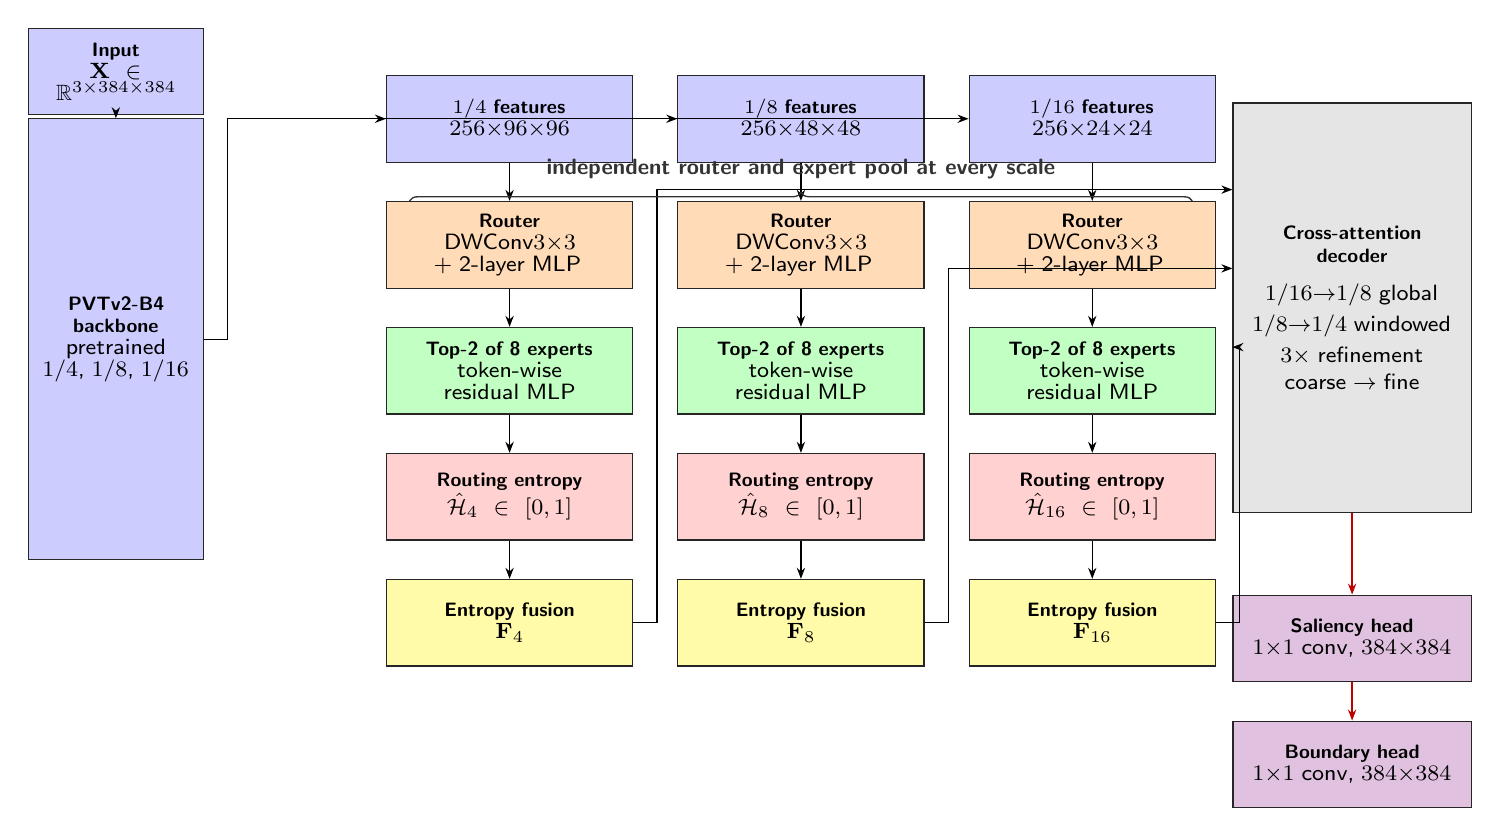
\begin{tikzpicture}[x=1mm,y=1mm, arr/.style={moeflow},
    lane/.style={moeblock, minimum width=31mm, text width=30mm, minimum height=11mm}]

% --- one lane per scale; boxes stacked vertically so each can stay large ---
\def\yF{32}\def\yR{16}\def\yE{0}\def\yH{-16}\def\yC{-32}
\def\xLaneA{50}\def\xLaneB{87}\def\xLaneC{124}
\def\xDec{157}

% input and backbone
\node[moeback, minimum width=22mm, text width=21mm, minimum height=11mm] (input) at (0,38)
  {\textbf{Input}\\ {\footnotesize$\bX\in\reals^{3\times384\times384}$}};
\node[moeback, minimum width=22mm, text width=21mm, minimum height=56mm] (bb) at (0,4)
  {\textbf{PVTv2-B4}\\ \textbf{backbone}\\ {\footnotesize pretrained}\\ {\footnotesize $1/4$, $1/8$, $1/16$}};

% --- lane 1/4 ---
\node[moeback, lane] (f4)  at (\xLaneA,\yF) {\textbf{$1/4$ features}\\ {\footnotesize $256{\times}96{\times}96$}};
\node[moerout, lane] (r4)  at (\xLaneA,\yR) {\textbf{Router}\\ {\footnotesize DWConv$3{\times}3$ + 2-layer MLP}};
\node[moeexp, lane]  (e4)  at (\xLaneA,\yE) {\textbf{Top-2 of 8 experts}\\ {\footnotesize token-wise residual MLP}};
\node[moeent, lane]  (h4)  at (\xLaneA,\yH) {\textbf{Routing entropy}\\ {\footnotesize $\Hs_4\in[0,1]$}};
\node[moefuse, lane] (c4)  at (\xLaneA,\yC) {\textbf{Entropy fusion}\\ {\footnotesize $\bF_4$}};

% --- lane 1/8 ---
\node[moeback, lane] (f8)  at (\xLaneB,\yF) {\textbf{$1/8$ features}\\ {\footnotesize $256{\times}48{\times}48$}};
\node[moerout, lane] (r8)  at (\xLaneB,\yR) {\textbf{Router}\\ {\footnotesize DWConv$3{\times}3$ + 2-layer MLP}};
\node[moeexp, lane]  (e8)  at (\xLaneB,\yE) {\textbf{Top-2 of 8 experts}\\ {\footnotesize token-wise residual MLP}};
\node[moeent, lane]  (h8)  at (\xLaneB,\yH) {\textbf{Routing entropy}\\ {\footnotesize $\Hs_8\in[0,1]$}};
\node[moefuse, lane] (c8)  at (\xLaneB,\yC) {\textbf{Entropy fusion}\\ {\footnotesize $\bF_8$}};

% --- lane 1/16 ---
\node[moeback, lane] (f16) at (\xLaneC,\yF) {\textbf{$1/16$ features}\\ {\footnotesize $256{\times}24{\times}24$}};
\node[moerout, lane] (r16) at (\xLaneC,\yR) {\textbf{Router}\\ {\footnotesize DWConv$3{\times}3$ + 2-layer MLP}};
\node[moeexp, lane]  (e16) at (\xLaneC,\yE) {\textbf{Top-2 of 8 experts}\\ {\footnotesize token-wise residual MLP}};
\node[moeent, lane]  (h16) at (\xLaneC,\yH) {\textbf{Routing entropy}\\ {\footnotesize $\Hs_{16}\in[0,1]$}};
\node[moefuse, lane] (c16) at (\xLaneC,\yC) {\textbf{Entropy fusion}\\ {\footnotesize $\bF_{16}$}};

% --- decoder ---
\node[moedec, minimum width=30mm, text width=29mm, minimum height=52mm] (dec) at (\xDec,8)
  {\textbf{Cross-attention}\\ \textbf{decoder}\\[1.5mm]
   {\footnotesize $1/16{\to}1/8$ global\\[0.6mm] $1/8{\to}1/4$ windowed\\[0.6mm]
    $3\times$ refinement\\[0.6mm] coarse $\to$ fine}};

% --- heads ---
\node[moehead, minimum width=30mm, text width=29mm, minimum height=11mm] (sal) at (\xDec,-34)
  {\textbf{Saliency head}\\ {\footnotesize $1{\times}1$ conv, $384{\times}384$}};
\node[moehead, minimum width=30mm, text width=29mm, minimum height=11mm] (bnd) at (\xDec,-50)
  {\textbf{Boundary head}\\ {\footnotesize $1{\times}1$ conv, $384{\times}384$}};

% --- arrows ---
\draw[arr] (input) -- (bb);
\def\dOut{3.0}
\draw[arr] (bb.east) -- ++(\dOut,0) |- (f4.west);
\draw[arr] (bb.east) -- ++(\dOut,0) |- (f8.west);
\draw[arr] (bb.east) -- ++(\dOut,0) |- (f16.west);
\foreach \a/\b in {f4/r4, r4/e4, e4/h4, h4/c4, f8/r8, r8/e8, e8/h8, h8/c8,
                   f16/r16, r16/e16, e16/h16, h16/c16}{
  \draw[arr] (\a) -- (\b);
}
\draw[arr] (c4.east)  -- ++(\dOut,0) |- ([yshift=15mm]dec.west);
\draw[arr] (c8.east)  -- ++(\dOut,0) |- ([yshift=5mm]dec.west);
\draw[arr] (c16.east) -- ++(\dOut,0) |- ([yshift=-5mm]dec.west);
\draw[arr, draw=red!75!black] (dec.south) -- (sal.north);
\draw[arr, draw=red!75!black] (sal.south) -- (bnd.north);

% --- one brace over the three routers, marking them independent ---
\draw[decorate, decoration={brace, amplitude=3pt}, black!80, line width=0.5pt]
  ([xshift=3mm]r4.north west) -- ([xshift=-3mm]r16.north east)
  node[midway, above=1.5mm, font=\sffamily\footnotesize\bfseries]
  {independent router and expert pool at every scale};

\end{tikzpicture}%
}
\moelegend

\clearpage
\section*{Figure 2 --- Routing mechanism}
\noindent
\centering
\resizebox{0.92\textwidth}{!}{%
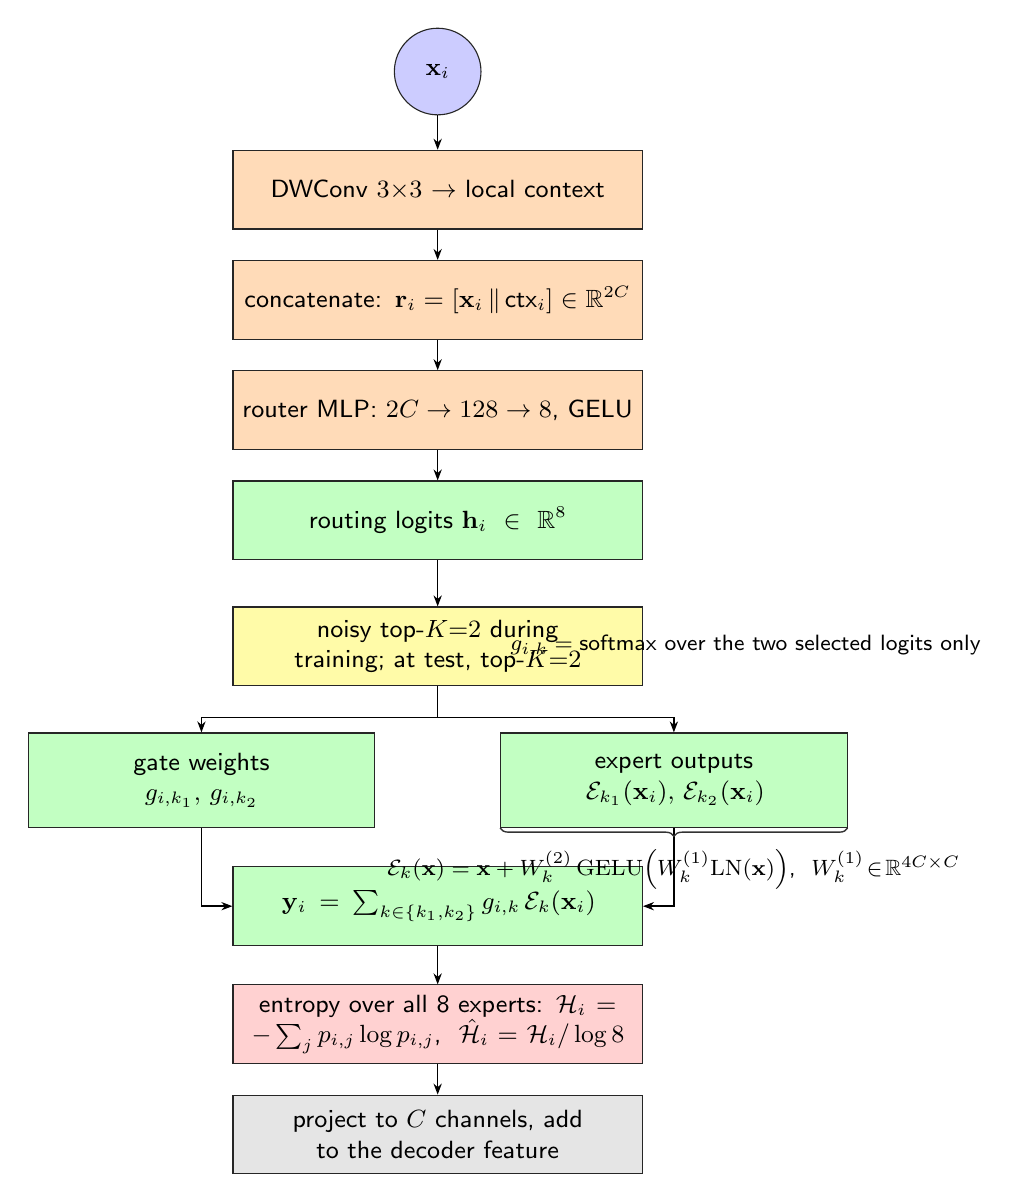
\begin{tikzpicture}[x=1mm,y=1mm,
  token/.style={circle, draw=black!85, line width=0.4pt, fill=blue!20,
    minimum size=11mm, font=\sffamily\small\bfseries, inner sep=0pt},
  op/.style={moerout, minimum width=52mm, text width=50mm, minimum height=10mm,
    font=\sffamily\small},
  logits/.style={moerout, minimum width=52mm, text width=50mm, minimum height=10mm,
    font=\sffamily\small, fill=green!24},
  exp/.style={moeexp, minimum width=44mm, text width=42mm, minimum height=12mm,
    font=\sffamily\small},
  dec/.style={moedec, minimum width=52mm, text width=50mm, minimum height=10mm,
    font=\sffamily\small},
  note/.style={font=\sffamily\footnotesize, anchor=west},
]

\node[token] (x)    at (0,0)    {$\bx_i$};
\node[op]    (ctx)  at (0,-15)  {DWConv $3{\times}3$ $\to$ local context};
\node[op]    (cat)  at (0,-29)  {concatenate: $\br_i=[\bx_i\,\|\,\text{ctx}_i]\in\reals^{2C}$};
\node[op]    (mlp)  at (0,-43)  {router MLP: $2C\to 128\to 8$, GELU};
\node[logits] (log) at (0,-57)  {routing logits $\bh_i\in\reals^{8}$};

\node[op, fill=yellow!34] (topk) at (0,-73)
  {noisy top-$K{=}2$ during training; at test, top-$K{=}2$};

% --- the two selected experts ---
\node[exp] (gk) at (-30,-90) {gate weights\\ $g_{i,k_1},\,g_{i,k_2}$};
\node[exp] (ek) at (30,-90)  {expert outputs\\ $\E_{k_1}(\bx_i),\,\E_{k_2}(\bx_i)$};
\node[op, fill=green!24] (sum) at (0,-106)
  {$\by_i=\textstyle\sum_{k\in\{k_1,k_2\}} g_{i,k}\,\E_k(\bx_i)$};

\node[op, fill=red!18] (ent) at (0,-121)
  {entropy over all 8 experts: $\mathcal{H}_i=-\sum_j p_{i,j}\log p_{i,j}$, \ $\Hs_i=\mathcal{H}_i/\log 8$};
\node[dec] (dec) at (0,-135) {project to $C$ channels, add to the decoder feature};

% --- arrows ---
\foreach \a/\b in {x/ctx, ctx/cat, cat/mlp, mlp/log, log/topk, sum/ent, ent/dec}{
  \draw[moeflow] (\a) -- (\b);
}
\draw[moeflow] (topk.south) -- ++(0,-4) -| (gk.north);
\draw[moeflow] (topk.south) -- ++(0,-4) -| (ek.north);
\draw[moeflow] (gk.south) |- (sum.west);
\draw[moeflow] (ek.south) |- (sum.east);

\node[note] at (8,-73) {$g_{i,k}=\text{softmax}$ over the two selected logits only};

\draw[decorate, decoration={brace, amplitude=3pt, mirror}, black!80, line width=0.5pt]
  (ek.south west) -- (ek.south east);
\node[font=\sffamily\footnotesize, below=1.5mm of ek, align=center]
  {$\E_k(\bx)=\bx+W_k^{(2)}\,\mathrm{GELU}\!\left(W_k^{(1)}\mathrm{LN}(\bx)\right)$,\ \ $W_k^{(1)}\!\in\!\reals^{4C\times C}$};

\end{tikzpicture}%
}

\end{document}
